\section{Infiltration - Part 2}
\subsection{Goal and Complexity}
\subsection*{Complexity: Beginner}

\subsection*{Prerequisites: None}

The goal of this tutorial is to get familiar with the $DRUtES$ standard Richards equation module and $DRUtES$ configuration in 1D by simulating infiltration into different soil \medskip

\subsection{Scenarios}

We use the same parameters as in the previous infiltration scenario (Tab. \ref{tab_inf1}). We assume a constant ponding depth at the top boundary.  Similar to the state of saturation in the previous scenario at the bottom boundary, where we knew the solution of the water table, we can assume the height of the water table, the ponding depth, to be defined with a Dirichlet condition, where the value is similar to the height of the ponding depth. At the bottom, we assume that only gravitational force acts on the bottom drainage. This also means that the pressure head gradient is zero. This boundary condition is called \textbf{free drainage}. The set-up of these scenarios are the same as in the previous infiltration scenarios, except for the boundary conditions. In these scenarios, we also want to investigate the effects on discretization, especially on the flux over the top boundary.  


\begin{figure}[!h]
\centering
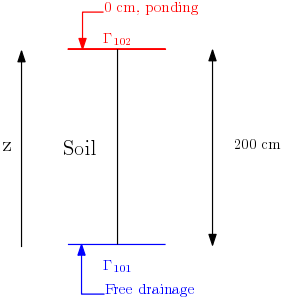
\includegraphics[width=5cm]{Fig_inf2/domain.png}
\caption{1D domain set-up of infiltration scenario with top and bottom boundary conditions. A constant ponding is assigned to the top, defined with a Dirichlet condition of 0 cm. Free drainage occurs at the bottom, which indicates that the pressure head gradient is 0 and water flows only due to gravity.}
\end{figure}

\newpage

\section*{Scenario 1}

Infiltration into sandy soil. 

$global.conf$: Choose correct model, dimension, time discretization and observation times.
\begin{enumerate}
\item Open \textbf{\emph{global.conf}} in a text editor of your choice. 
\item Model type: Your first input is the module. Input is \textbf{RE}.
\item Initial mesh configuration \begin{enumerate}
\item The dimension of our problem is 1. Input: 1.
\item We use the internal mesh generator. Input: 1. 
\end{enumerate}
\item Error criterion \begin{enumerate} 
\item Maximum number of iteration of the Picard method: 20 
\item h tolerance: 1e-1.
\end{enumerate}
\item Time information 
\begin{enumerate} 
%\item integration method is 3 point formula. Input: 30. 
\item Time units are in hours: input d
\item Initial time: 1e-4.
\item End time: 1.
\item Minimum time step: 1e-4.
\item Maximum time step: 0.1.
\end{enumerate}
\item Observation time settings \begin{enumerate}
\item Observation time method: 2
\item Set file format of observation: pure. Output in 1D is always in raw data. Different options will not impact output in 1D.
\item Make sequence of observation time: n
\item Number of observation times: 10
\item Observation time values: 0.001,
0.005,
0.01,
0.05,
0.1,
0.2,
0.3,
0.4,
0.6,
0.8. Use a new line for each input. \textit{DRUtES} automatically generates output for the initial time and final time. DRUtES will generate 12 output files, e.g. \textit{RE\_matrix\_press\_head-x.dat}, \textit{RE\_matrix\_theta-x.dat} where x is the number of the file and not the output time. The initial time is assigned an x value of 0. 
\end{enumerate}
\item Observation point settings \begin{enumerate}
\item Observation point coordinates: 0, 200. Use a new line for each input. \textit{DRUtES} will generate 2 output files, e.g. \textit{obspt\_RE\_matrix-1.out}, where x is the ID of the observation point. 
\end{enumerate}
\item Ignore other settings for now. 
\item Save $global.conf$
\end{enumerate}


$drumesh1D.conf$: Mesh definition, i.e. number of materials and spatial discretization
\begin{enumerate}
\item Open \textbf{\emph{drumesh1D.conf}} in a text editor of your choice. 
\item Geometry information: 200 cm - domain length
\item Amount of intervals: 1
\item
\adjustbox{max height=\dimexpr\textheight-5cm\relax,
           max width=\textwidth}{
\small\begin{tabular}{|c | c | c|}
\hline
density & bottom & top \\
 \hline
5 & 0 & 200\\
\hline
\end{tabular}
}
\item number of materials: 1
\item \adjustbox{max height=\dimexpr\textheight-5cm\relax,
           max width=\textwidth}{
\small\begin{tabular}{|c | c | c|}
\hline
id & bottom & top \\
 \hline
5 & 0 & 200 \\
\hline
\end{tabular}
}
\end{enumerate}

\emph{matrix.conf}: Configuration file for water flow 


\begin{enumerate}
\item Open \emph{matrix.conf} in a text editor of your choice. 
\item How-to use constitutive relations? [integer]: 1
\item Length of interval for precalculating the constitutive functions: 200
\item Discretization step for constituitive function precalculation: 0.1
\item number of soil layers [integer]: 1
\item \adjustbox{max height=\dimexpr\textheight-5cm\relax,
	max width=\textwidth}{
	\small\begin{tabular}{|c | c | c|c | c | c|}
		\hline
		alpha & n & m & theta\_r & theta\_s & specific storage\\
		\hline
		0.1 & 2.2  & 0.55 & 0.00 & 0.40  &0  \\
		\hline
	\end{tabular}
}
\item The angle of the anisotropy determines the angle of the reference coordinate system. 0 means vertical flow. Anisotropy description. Anisotpropy description and hydraulic conductivity\\ \adjustbox{max height=\dimexpr\textheight-5cm\relax,
	max width=\textwidth}{
	\small\begin{tabular}{|c | c |}
		\hline
		angle [degrees] & K\_11  \\
		\hline
		0 & 400  \\
		\hline
	\end{tabular}
}
\item sink(-) /source (+) term per layer: 0
\item Initial condition is a constant pressure head of -200 cm across the soil. \\ \adjustbox{max height=\dimexpr\textheight-5cm\relax,
	max width=\textwidth}{
	\small\begin{tabular}{|c | c | c|c |}
		\hline
		 init. cond [real] & type of init. cond &RCZA method [y/n] &  RCZA method val.  \\
		\hline
		   -200.0           &            hpres                       & n		   &          0 \\
		\hline
	\end{tabular}
}
\item number of boundaries: 2
\item \adjustbox{max height=\dimexpr\textheight-5cm\relax,
	max width=\textwidth}{
	\small\begin{tabular}{|c | c | c|c |}
		\hline
		boundary ID& boundary type   & use rain.dat [y/n]   & value  \\
		\hline
	101    &                   3        &           n        &        0.0 \\
	102             &          1         &          n         &       0.0        \\
	
		\hline
	\end{tabular}
}
\item Save matrix.conf.

\end{enumerate}

\section*{Run scenario 1}
Run the simulation in the terminal console.
\begin{enumerate}
\item Make sure you are in the right directory. 
\item To execute $DRUtES$: \\
\$ bin/drutes
\item After the simulation finishes, to generate png plots execute provided R script: \\
\$ Rscript drutes.conf/water.conf/waterplots.R -name sand
\item The output of the simulation can be found in the folder out
\end{enumerate}

\section*{Scenario 2}
Infiltration into silty soil
\begin{enumerate}
\item \emph{global.conf} and \emph{drumesh1D.conf} remain the same.
\item Open \emph{matrix.conf} in a text editor of your choice. 
\item Use the same set-up, but change the van Genuchten parameters to:
\item \adjustbox{max height=\dimexpr\textheight-5cm\relax,
	max width=\textwidth}{
	\small\begin{tabular}{|c | c | c|c | c | c|}
		\hline
		alpha & n & m & theta\_r & theta\_s & specific storage\\
		\hline
		0.08 & 1.8   & 0.44 & 0.05 & 0.45  & 0 \\
		\hline
	\end{tabular}
}
\item anisothprophy description and hydraulic conductivity\\ \adjustbox{max height=\dimexpr\textheight-5cm\relax,
	max width=\textwidth}{
	\small\begin{tabular}{|c | c |}
		\hline
		angle [degrees] & K\_11  \\
		\hline
		0 & 40  \\
		\hline
	\end{tabular}
}
\item Save matrix.conf.
\end{enumerate}

\section*{Run scenario 2}
Run the simulation in the terminal console.
\begin{enumerate}
\item To execute $DRUtES$: \\
\$ bin/drutes
\item generate png plots with R script: \\
\$ Rscript drutes.conf/water.conf/waterplots.R -name silt
\end{enumerate}

\section*{Scenario 3}
Infiltration into clay soil
\begin{enumerate}
\item \emph{global.conf} and \emph{drumesh1D.conf} remain the same.
\item Open \emph{matrix.conf} in a text editor of your choice. 
\item Use the same set-up, but change the van Genuchten parameters to:
\item \adjustbox{max height=\dimexpr\textheight-5cm\relax,
	max width=\textwidth}{
	\small\begin{tabular}{|c | c | c|c | c | c|}
		\hline
		alpha & n & m & theta\_r & theta\_s & specific storage\\
		\hline
		0.01 & 1.5  & 0.33 & 0.1& 0.5   &0 \\
		\hline
	\end{tabular}
}
\item anisothprophy description and hydraulic conductivity\\ \adjustbox{max height=\dimexpr\textheight-5cm\relax,
	max width=\textwidth}{
	\small\begin{tabular}{|c | c |}
		\hline
		angle [degrees] & K\_11  \\
		\hline
		0 & 4  \\
		\hline
	\end{tabular}
}
\item Save matrix.conf.
\end{enumerate}

\section*{Run scenario 3}
Run the simulation in the terminal console.
\begin{enumerate}
\item To execute $DRUtES$: \\
\$ bin/drutes
\item generate png plots with R script: \\
\$ Rscript drutes.conf/water.conf/waterplots.R -name clay
\end{enumerate}

\section*{Tasks}

\begin{enumerate}
\item Describe the infiltration fronts for sand, silt and clay.
\item The results do not look very smooth. This is because of insufficient discretization. Improve the discretization for sand. With what set-up are the results better? Possibilities are: 
\begin{itemize}
\item in global.conf: Decrease the pressure head tolerance, Decrease the initial time step, Decrease the maximum time step.
\item in drumesh1D.conf: Decrease the mesh density. 
\end{itemize}
\item Why is the flux at the top so huge in the beginning?
\end{enumerate}



\section*{Results}

\subsection*{Task 1}
In the following time series of the infiltration into sand, silt and clay are presented. The infiltration front has moved furthest in sand, followed by silt and then clay. This is because of the assigned boundary conditions. The flux into sandy soil is very large. However, the time series show the numerical approximation is insufficient, especially for sand. This is because sand is the numerically most difficult to model as it has the steepest retention properties (largest n and largest alpha).

\begin{figure}[!h]
\centering
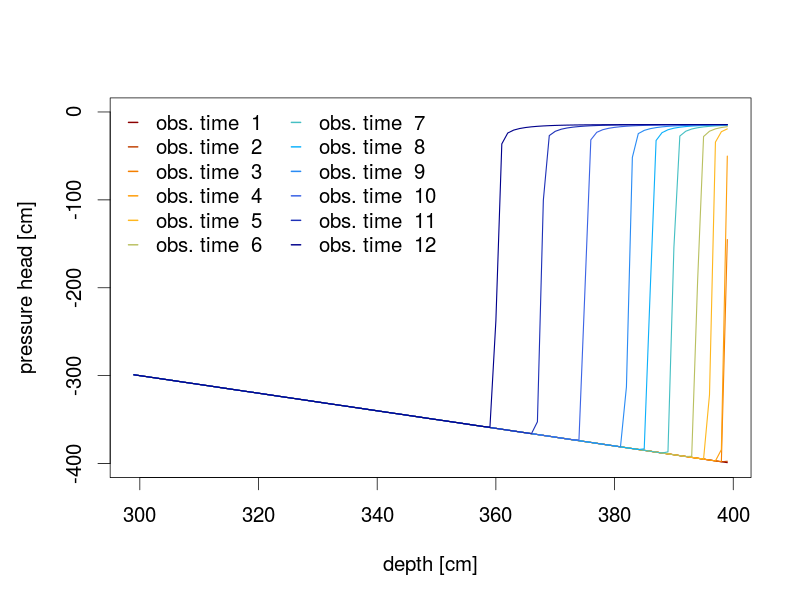
\includegraphics[width=0.49\textwidth]{Fig_inf2/obs_press_head_sand.png}
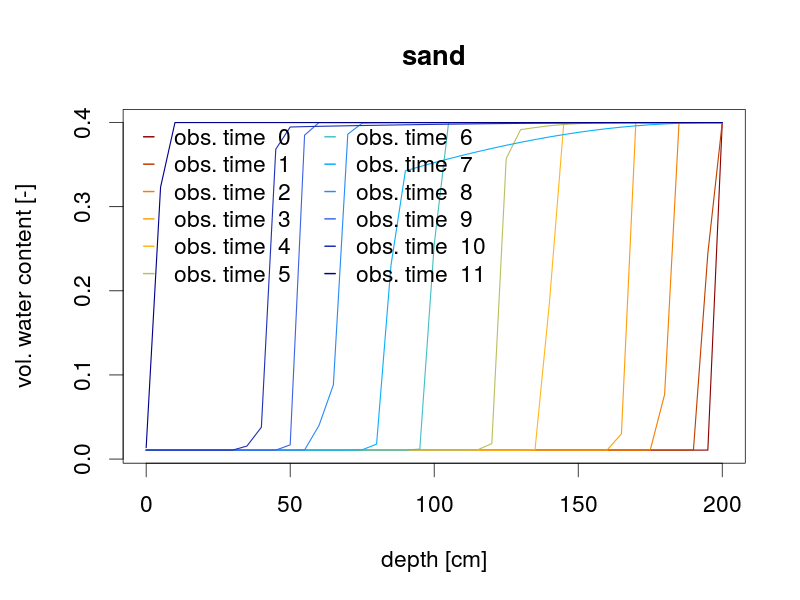
\includegraphics[width=0.49\textwidth]{Fig_inf2/obs_water_sand.png}
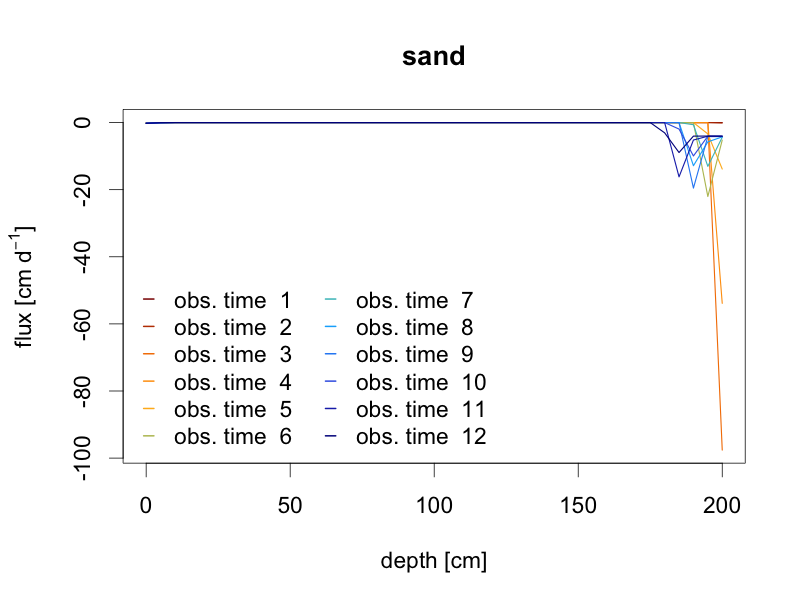
\includegraphics[width=0.49\textwidth]{Fig_inf2/obs_flux_sand.png}
\caption{Observation time series of pressure head, vol. water content and flux of infiltration into sand.}
\end{figure}

\begin{figure}[!h]
\centering
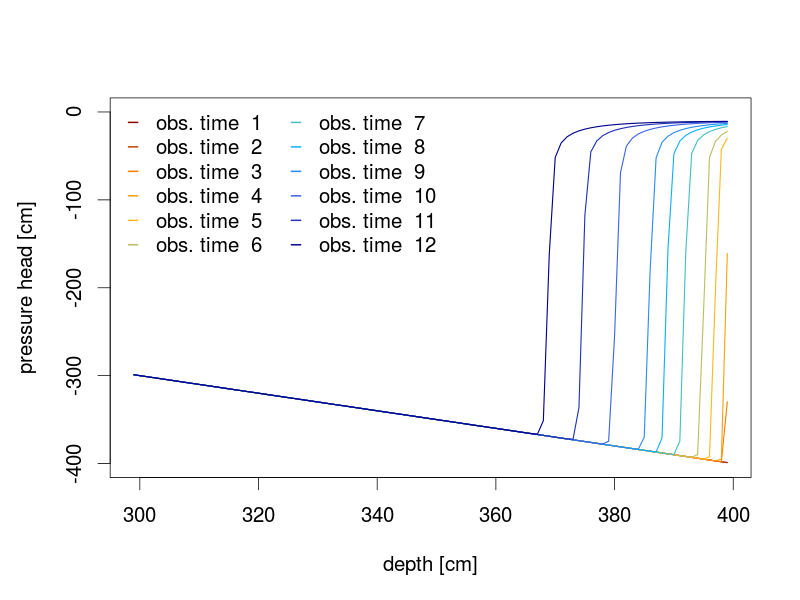
\includegraphics[width=0.49\textwidth]{Fig_inf2/obs_press_head_silt.png}
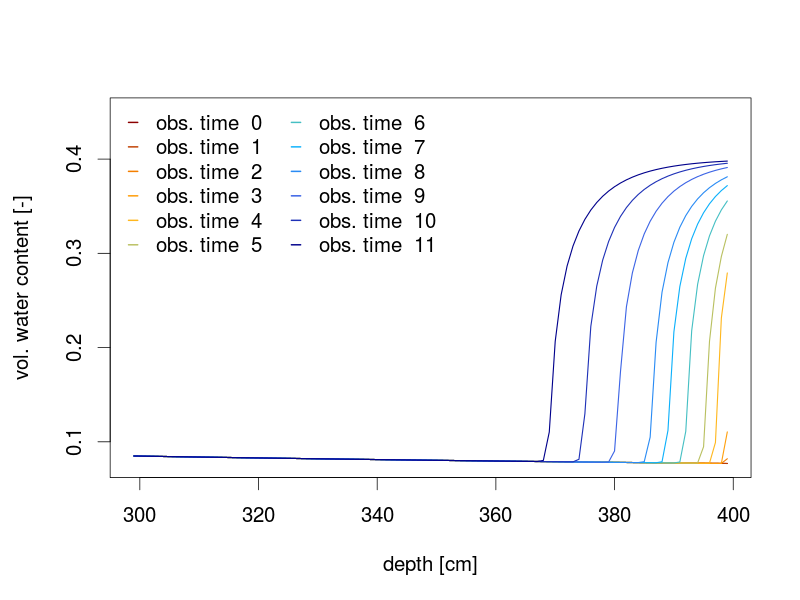
\includegraphics[width=0.49\textwidth]{Fig_inf2/obs_water_silt.png}
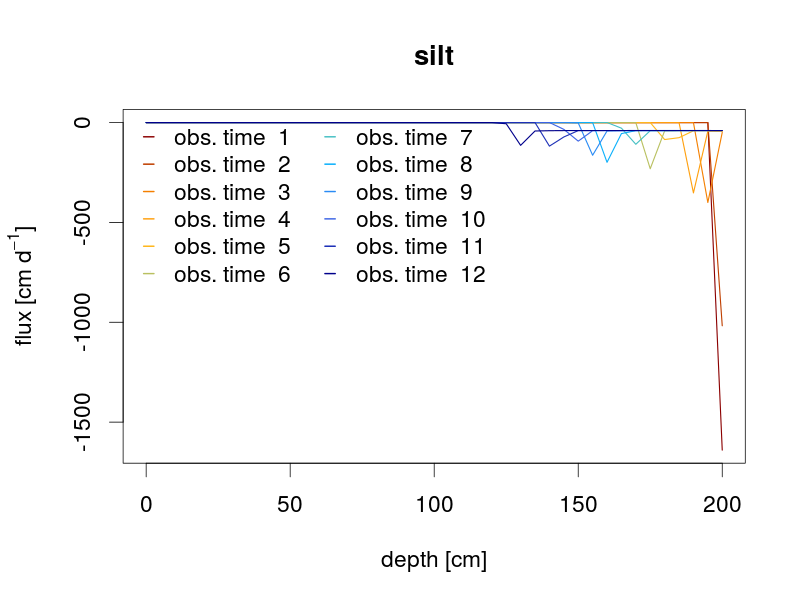
\includegraphics[width=0.49\textwidth]{Fig_inf2/obs_flux_silt.png}
\caption{Observation time series of pressure head, vol. water content and flux of infiltration into silt.}

\end{figure}


\begin{figure}[!h]
\centering
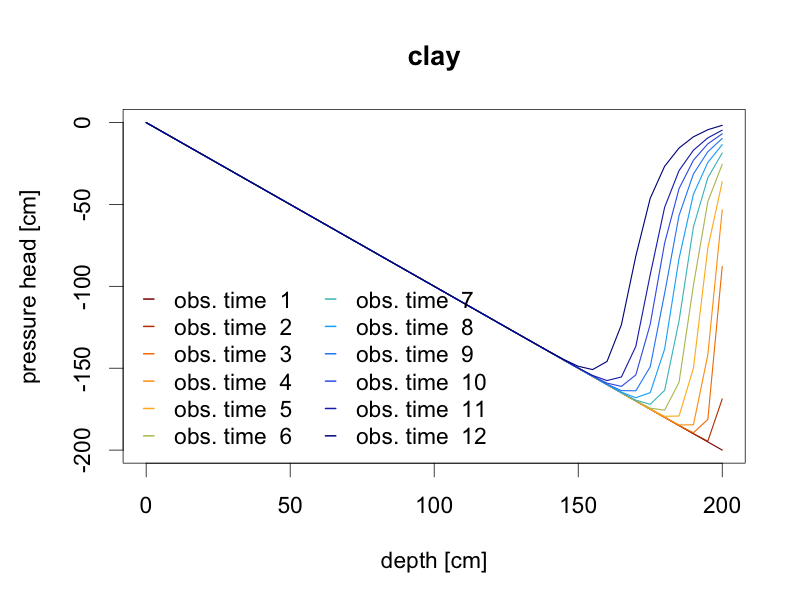
\includegraphics[width=0.49\textwidth]{Fig_inf2/obs_press_head_clay.png}
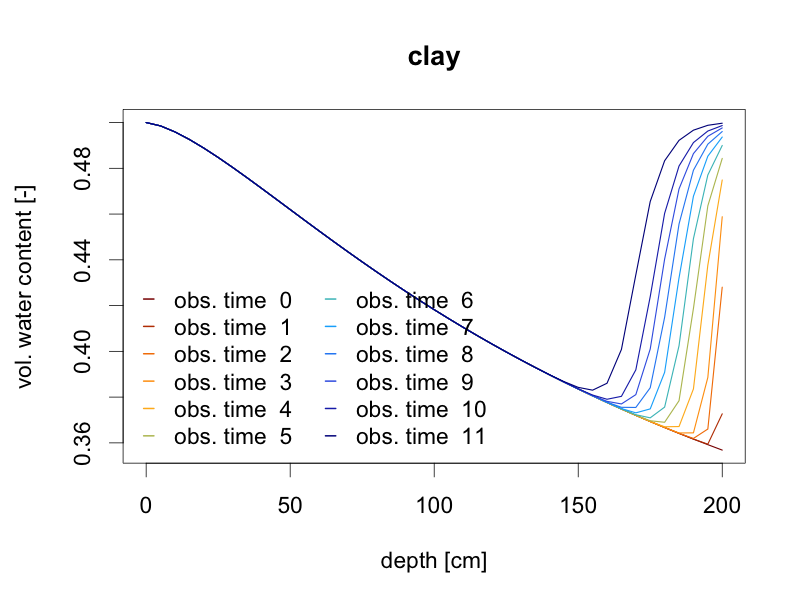
\includegraphics[width=0.49\textwidth]{Fig_inf2/obs_water_clay.png}
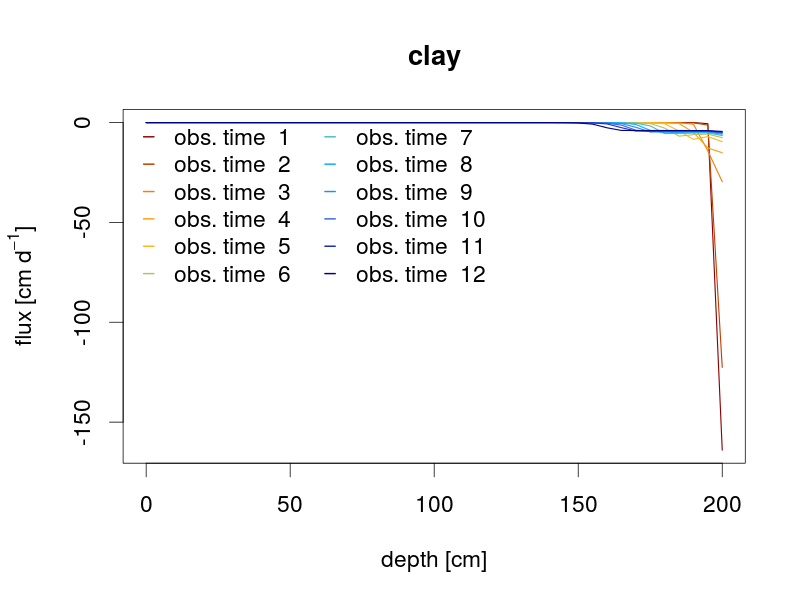
\includegraphics[width=0.49\textwidth]{Fig_inf2/obs_flux_clay.png}
\caption{Observation time series of pressure head, vol. water content and flux of infiltration into clay.}

\end{figure}

\newpage
\newpage
\subsection*{Task 2}

The solution for sand the water content and hydraulic pressure become a lot smoother with finer spatial discretization, eg. dz=0.5 and a finer temporal discretization by setting the lower minimal time step to 0.01. The fluxes are still spiky, but correlate with the infiltration front. Different solutions can be found by decreasing the minimal time step even further and also the h tolerance criterion. This, however, increases the simulation time substantially. For a reliable solution, the numerical solution should converge. This means that decreasing the time step, or discretization, should not lead to an entirely different solution. We notice, that reducing the h tolerance criterion improves the solution locally, but that reducing the maximum time step changes the depth of the infiltration front. This is because the mass balance is very much connected to the temporal discretization.

\begin{figure}[!h]
	\centering
	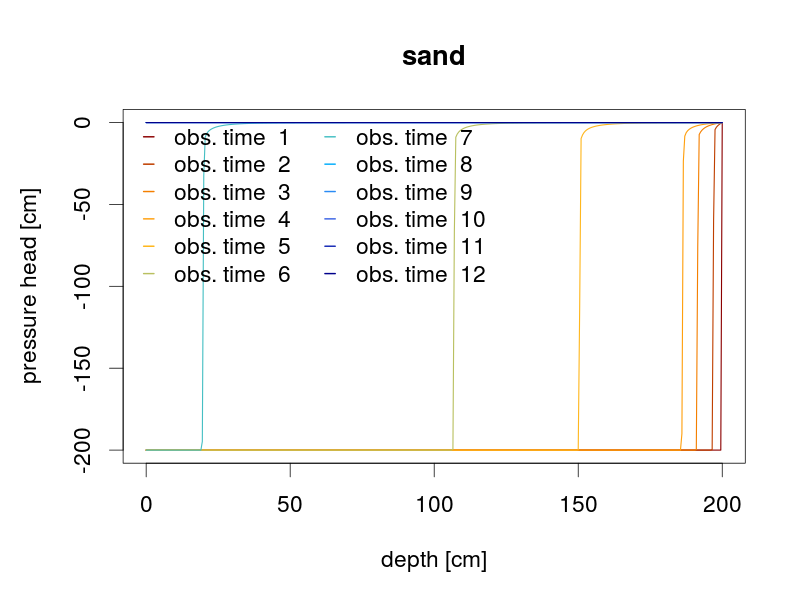
\includegraphics[width=0.49\textwidth]{Fig_inf2/obs_press_head_sand6.png}
	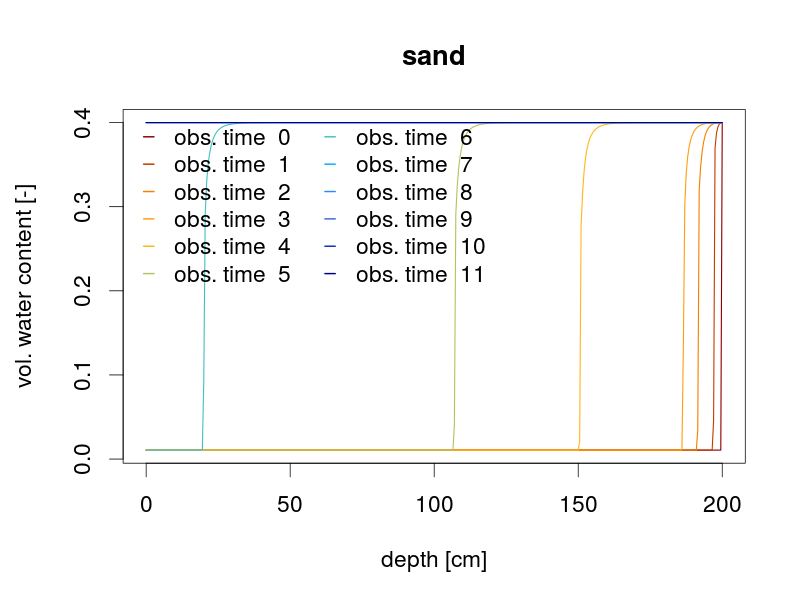
\includegraphics[width=0.49\textwidth]{Fig_inf2/obs_water_sand6.png}
	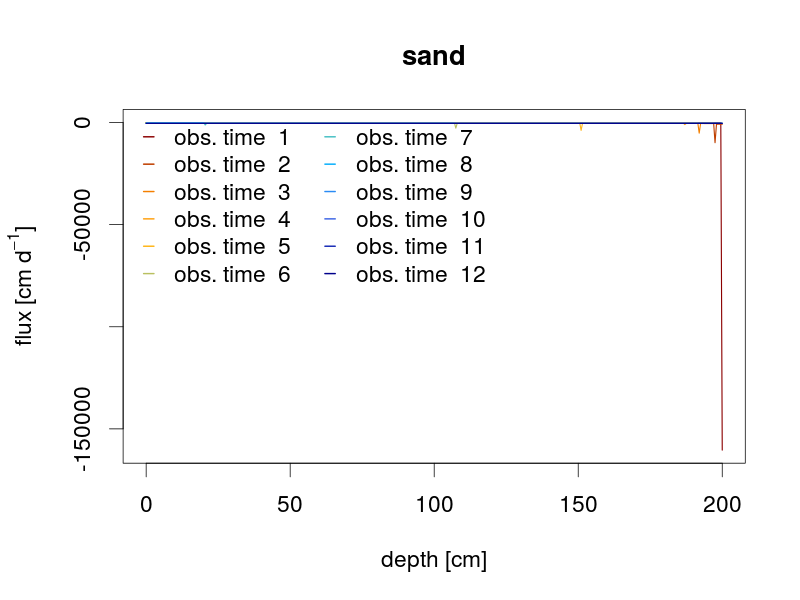
\includegraphics[width=0.49\textwidth]{Fig_inf2/obs_flux_sand6.png}
	\caption{Observation time series of pressure head, vol. water content and flux of infiltration into sand with improved discretization.}
\end{figure}

\subsection*{Task 3}
With the initial set-up, the flux at the top in sand is 15000 cm d$^{-1}$ in the beginning of the simulation. For silt, the flux was numerically calculated to be at 1500 cm d$^{-1}$ and for clay at 150 cm d$^{-1}$. The flux estimation becomes a lot larger with finer spatial discretization.

 This is due to the large hydraulic gradient between the saturated top boundary and the next node of $\nabla h=\frac{-200-0~}{\mathrm{dz}}$. The smaller the nodal distance dz is, the greater is the gradient. According to the Darcy-Buckingham law, the flux is proportional to the hydraulic conductivity. The hydraulic conductivity is highest for sand. This is why the flux is largest for sand and lowest for clay.
\newpage
\newpage
\newpage
\newpage
\subsection{Outcome}
\begin{enumerate}
\item You got familiar with the $DRUtES$ standard Richards Equation modules in 1D.
\item You understand basic parameterization of a typical sand, silt and clay with the van Genuchten-Mualem model.
\item You simulated infiltration in different soils.
\item You understand the term \emph{Free drainage} and \emph{initial condition}.
\item You understand the effects of different discretizations.
\end{enumerate}
